\documentclass[english,twoside,censored,tkt]{HYthesisML}

% In theses, open new chapters only at right page.
\PassOptionsToClass{openright,twoside,a4paper}{report}
\usepackage{csquotes}
\usepackage{comment}

%%%%%%%%%%%%%%%%%%%%%%%%%%%%%%%%%%%%%%%%%%%%%%%%%%%%%%%%%
%% REFERENCES
%% Some notes on bibliography usage and options:
%% natbib -> you can use, e.g., \citep{} or \parencite{} for (Einstein, 1905); with APA \cite -> Einstein, 1905 without ()
%% maxcitenames=2 -> only 2 author names in text citations, if more -> et al. is used
%% maxbibnames=99 as no great need to suppress the biliography list in a thesis
%% for more information see biblatex package documentation, e.g., from https://ctan.org/pkg/biblatex 

%% Reference style:
%% for numeric = Vancouver style -> [1] use:
\usepackage[style=numeric,bibstyle=numeric,backend=biber,natbib=true,maxbibnames=99,giveninits=true,uniquename=init]{biblatex}

\addbibresource{bibliography.bib}
% in case you want the final delimiter between authors & -> (Einstein & Zweistein, 1905) 
% \renewcommand{\finalnamedelim}{ \& }
% List the authors in the Bibilipgraphy as Lastname F, Familyname G,
\DeclareNameAlias{sortname}{family-given}
% remove the punctuation between author names in Bibliography 
%\renewcommand{\revsdnamepunct}{ }


%% Block of definitions for fonts and packages for picture management.
%% In some systems, the figure packages may not be happy together.
%% Choose the ones you need.

%\usepackage[utf8]{inputenc} % For UTF8 support, in some systems. Use UTF8 when saving your file.

\usepackage{lmodern}         % Font package, again in some systems.
\usepackage{textcomp}        % Package for special symbols
\usepackage[pdftex]{color, graphicx} % For pdf output and jpg/png graphics
\usepackage{epsfig}
\usepackage{subfigure}
\usepackage[pdftex, plainpages=false]{hyperref} % For hyperlinks and pdf metadata
\usepackage{fancyhdr}        % For nicer page headers
\usepackage{tikz}            % For making vector graphics (hard to learn but powerful)
%\usepackage{wrapfig}        % For nice text-wrapping figures (use at own discretion)
\usepackage{amsmath, amssymb} % For better math

\singlespacing               %line spacing options; normally use single

\fussy
%\sloppy                      % sloppy and fussy commands can be used to avoid overlong text lines
% if you want to see which lines are too long or have too little stuff, comment out the following lines
% \overfullrule=1mm
% to see more info in the detailed log about under/overfull boxes...
% \showboxbreadth=50 
% \showboxdepth=50

\title{Enabling knowledge retention in a machine learning big data system: a case study}

% TM: Contributors to template editors now listed in the beginning of the file in comments
\author{Riikka Korolainen}
\date{\today}

% Set supervisors and examiners, use the titles according to the thesis language
% Prof. 
% Dr. or in Finnish toht. or tri or FT, TkT, Ph.D. or in Swedish... 
\supervisors{Prof.~D.U.~Mind, Dr.~O.~Why}
\examiners{Prof.~D.U.~Mind, Dr.~O.~Why}


\keywords{machine learning, lifelong learning, internet of things, maritime}
\additionalinformation{\translate{\track}}

%% Use 1-3 paths, and use right arrows between the
%% about three levels in the path; each path requires a new line.

\classification{\protect{\ \\
\  General and reference $\rightarrow$ Document types  $\rightarrow$ Surveys and overviews\  \\
\  Applied computing  $\rightarrow$ Document management and text processing  $\rightarrow$ Document management $\rightarrow$ Text editing
}}

%% if you want to quote someone special. You can comment this line out and there will be nothing on the document.
%\quoting{Bachelor's degrees make pretty good placemats if you get them laminated.}{Jeph Jacques}


%% OPTIONAL STEP: Set up properties and metadata for the pdf file that pdfLaTeX makes.
%% Your name, work title, and keywords are recommended.
\hypersetup{
    unicode=true,           % to show non-Latin characters in Acrobat’s bookmarks
    pdftoolbar=true,        % show Acrobat’s toolbar?
    pdfmenubar=true,        % show Acrobat’s menu?
    pdffitwindow=false,     % window fit to page when opened
    pdfstartview={FitH},    % fits the width of the page to the window
    pdftitle={Big data system architectures for performance: a Comparison},            % title
    pdfauthor={Riikka Korolainen},           % author
    pdfsubject={},          % subject of the document
    pdfcreator={},          % creator of the document
    pdfproducer={pdfLaTeX}, % producer of the document
    pdfkeywords={machine learning} {sensor data}, % list of keywords for
    pdfnewwindow=true,      % links in new window
    colorlinks=true,        % false: boxed links; true: colored links
    linkcolor=black,        % color of internal links
    citecolor=black,        % color of links to bibliography
    filecolor=magenta,      % color of file links
    urlcolor=cyan           % color of external links
}

\begin{document}

\maketitle

\begin{abstract}

A common problem with creating successful large-scale machine learning systems is the fact that significant effort is needed to keep the system working over long periods of time. This is mainly caused by unpreparedness to changes in the data source, a phenomenon known as concept drift. In order to adapt to these drifts, advanced and case-tailored maintenance schemes are needed.

This thesis searches for efficient model updating schemes to bring machine learning to the maritime domain, to applications such as traffic forecasting. Given the model type, recurrent neural networks, and case-specific requirements, such as large data and comparatively loose end-to-end latency requirements, the optimal drift-coping methods are searched for.

Based on literature, it is found that monitoring both models and data, optimizing neural network training using data parallelism and network approximation, and versioning data with an identifier-based mechanism would most likely enable consistent accuracy of the models despite environmental changes. However, it is found that for many approaches, the usability for the specific case cannot be determined without the experimental benchmarking of several options.
%some abstract drafting... (what to include)
% essence of your paper
% prepares readers to follow
%  remember key points
  
%  the context - maritime
%  the general topic under study - big data processing systems
%  the specific topic of your research - updating neural networks efficiently
%  the central questions or statement of the problem your research addresses - which updating workflow is optimal for facilitating model maintenance
%  what’s already known about this question, what previous research has done or shown - showed a lot of options for how models can stay up to date with concept drift in very specific situations
%  motivation - in order to bridge the gap between research and industry, the applicability of approaches need to be studied
%  your research and/or analytical methods - literature based
%  your main findings, results, or arguments - that neural networks can be kept up to date with highly voluminous data using explicit concept drift detection, model approximation / parallelization and batch size increasing
%  implication - what needs to be taken into account when choosing the optimal updating workflow



\end{abstract}

\newpage
\mytableofcontents
\mainmatter

%%%%%%%%%%%%%%%%%%%%%%%%%%%%%%%%%%%%%%%%%%%%%%%%%%%%%%%%%
%% STEP 4: Write the thesis.
%%%%%%%%%%%%%%%%%%%%%%%%%%%%%%%%%%%%%%%%%%%%%%%%%%%%%%%%%
%% Your actual text starts here. You shouldn't mess with the code above the line except
%% to change the parameters. Removing the abstract and ToC commands will mess up stuff.
%%
%% You may wish to include material to avoid browsing the definitions
%% above. Command \include{file} includes the file of name file.tex.
%% As a side effect, subsequent inclusions may force a page break.

\chapter{Introduction}
% 1st sect: GENERAL BACKGROUND: data environments evolve. data stream processing requires being accurate efficiently.
A problem occurring in nearly every application of machine learning is the challenge of handling evolving environments, a problem known as concept drift. Meanwhile, the domain of data stream processing proposes its own set of challenges, the main one being the ability of providing accurate predictions at any time despite large volumes of data and constrained time and memory resources. The combination of these two problems, the need to adapt to evolving data while meeting the systems requirements, is complex, but common.

% there are lots of solutions to this so requirements are needed to select from them
Multitudes of approaches have been proposed as a solution to the problem of handling concept drift efficiently in stream processing systems, each with their own set of strengths. Therefore, to be able to compare the applicability of these solutions, a set of requirements should be used as a starting point. A case study is presented for this purpose, and the solution is searched for given the set of identified assumptions and requirements. 

% the context intro
The thesis at hand uses as context an on-going research project, VesselAI, aiming for applying novel machine learning to the domain of maritime. The domain in question is characteristic in the especially large volume of incoming sensor data and the slowness of vessel traffic in comparison. Additional context specifics include low-quality and heterogeneousness of data, the complexity and novelty of the deep learning models used, and the delayedness of model feedback. 

% goal
The goal of this analysis is, given the project context, to find the most optimal approach for maintaining model accuracy. In other words, from the challenges identified in the VesselAI state-of-the-art analysis \cite{D1.1}, the problem tackled is `ML model retraining is computationally very heavy: in environments where data evolves, it is urgent to use architectures that manage ML models in order to adapt to new data/tasks and retrain when necessary'. In addition to the suggested approach of lifelong learning, additional insight is gathered from the research fields of concept drift adaptation, batch learning, and AutoML.  This way literature gap of works addressing the maritime domain and automated model adaptation identified in \cite{D1.1} is addressed.   

% systems perspective
Traditionally, works addressing the problem of concept drift largely focus on how to build a model that is able to adapt to the changing environment. This thesis can, from this perspective, also be seen as a systems approach to concept drift. If a model is taken as given, it is discussed how the system organization would be able to make sure the model stays accurate. This perspective also aims to take into account the insight on best practices from the field of designing big data systems. From the lessons learned there it is especially aimed for a solution that is simple and mature enough to be applied to a real-world scenario.

% 2nd section: RESEARCH Q'S, METHODOLOGY, RESULTS SUMMARY

% outline
% main question
% exact definitions of main question
% sub-questions
% note on methodology (literature based but not systematic, non-empirical)
% results summary

% comment: the sentence on the model is a little vague, tailored means that it is made for the case not just taken from somewhere else. I'm unsure what words to mention on the model here.

% research question
The main research question addressed in this work is the following:

\begin{center}
    Given the domain context and the models used, how to organize a workflow for efficient updating of the models in order to meet the demands posed by the use case?
\end{center}

As further elaboration, by updating the model it is meant that the model parameters are changed. By efficient we mean efficiency relative to the data volume, not relative to computing resources. This means that an average high performance cluster is assumed and the target is to be able to utilise that to be able to handle as much data in as little time as possible. The domain context used is the maritime domain, and the model used is assumed to be a deep learning model operating in batch mode.

The secondary research questions considered as implications of the primary one are the following:

\begin{itemize}
    \item Is it possible to organize retraining effectively enough to handle incoming data, or does the model itself need to be adaptable?
    \item How much human intervention is required for maintaining the updating schemes; what are the possibilities of automating these workflows?
\end{itemize}

% add paragraph on results here later...

As a note on methodology, the investigation in its entirety is based on literature. Conducting a systematic literature review would be beyond the scope of this thesis, so only material directly relevant regarding the specific set of requirements is taken into account. Testing the various approaches in practice is also beyond scope; the empirical investigation of these findings is left to future works. This limits both the set of options considered to those already used in the problem domain and the evaluation to analyzig the thoroughness of existing evidence in literature.

% 3rd section: CHAPTER ROLES
% if the result is so that multiple can be good then change chap 4 description to state that the systems applying the max two best seeming options are presented.

The rest of this thesis is organized as follows:

Chapter 2 presents the necessary background knowledge to the reader: an overview of the general organization of a big data system, definitions in the field of machine learning model updating, and an introduction to the maritime domain. Chapter 3 analyzes the various model updating approaches presented previously and discusses which approaches would be most useful given the context of the case. Then, ways of automating the optimal-seeming approaches are shortly discussed. Chapter 4 synthesizes the findings above and presents an abstract overview of the system that would apply the optimal updating workflow. In addition it is discussed how certain these findings are given the quality and thoroughness of the literature used. The thesis is concluded with discussion on the applicability of the results achieved to similar problems from different domains.

\chapter{Overview on large-scale machine\\ learning systems for maritime}

% in case a neural networks introduction is needed: \cite{ben-nun_demystifying_2019} sect 4.1 has a good description

% ingressi: mitä aiot rakentaa luvussa, mikä tulee esille, miksi se on tärkeää, mihin tällä kokonaisuudella pyritään

The general task of big data systems is that they should be able to handle vast amounts of data and from that be able to provide predictions in a timely manner. To position our problem of model maintenance in this larger domain, this chapter provides an introduction to the necessary background. First, the entire big data pipeline is presented on an abstract level, alongside best practices of systems design. Then, to clarify the terminology, machine learning approaches for efficient model updates are defined. Lastly, the requirements of the case used to compare the maintenance approaches are derived from the application domain description.

\section{Introduction to big data systems}

% MLOps is a term that should be used / mentioned somewhere

% current main concern for this sect: I state out a lot of facts without giving a reference -> the fine line between common knowledge and what needs backing...

% add here: this system presented is a ml one, some notes added specifically on the usage of neural networks in these systems

\subsection{The high-level components}

% add here: eg DATE n kung fu papers (1st & 2nd from lucy) state that in ML systems distribution is of high importance. add to model training part
%kungfu: stochastic gradient descent (SGD) algorithm is common, give that as an example maybe?

% the automl survey can be ref'd here. add here a note on what automl + possibly mlops is.

% maybe add: model development. in neural networks neural architecture search is a major computational problem that has a lot of automl research attention. however, this operation is only needed when the model is first developed, not during updates, so its optimization is not considered

The steps that most large-scale machine learning systems compose of are displayed in the following figure: 

% the figure is too small... -> not very readable
\begin{figure}[ht]
%\begin{figure}[tbh] t= top, b = bottom, h=here
\ \newline
\begin{center}
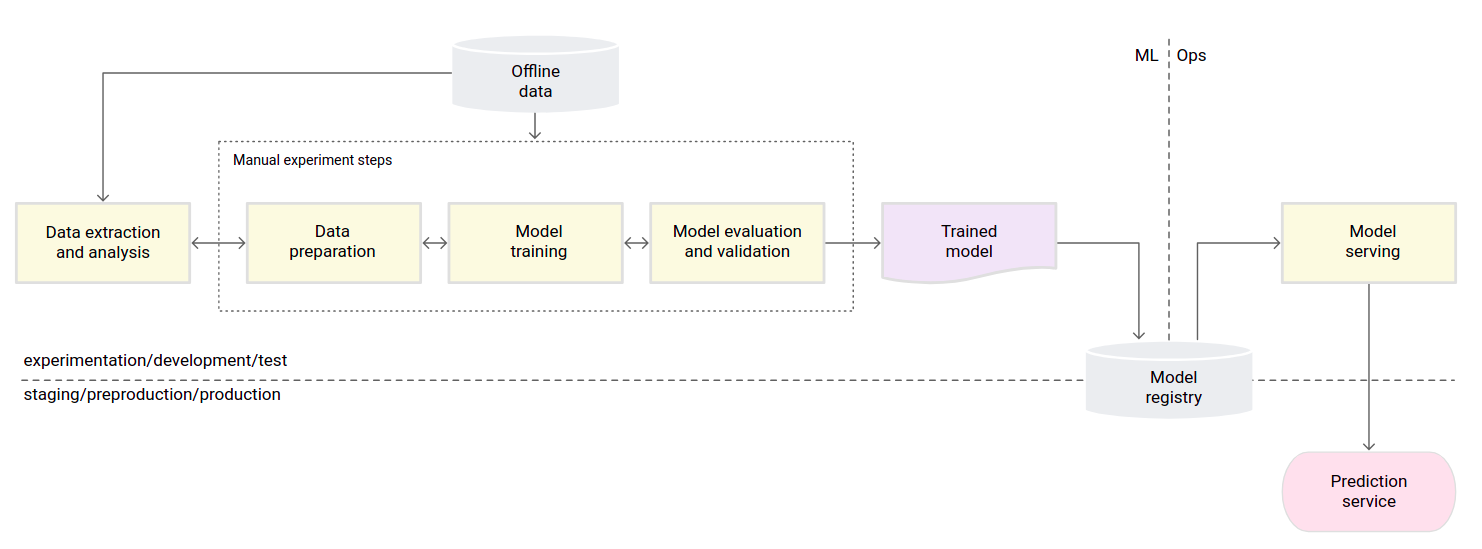
\includegraphics[width=0.9\textwidth]{simplegoogle.png}
\caption{Abstract components of a big data analytics system. From Google Developer MLOps guide~\cite{googlemlops}.}
\label{simplepipeline}
\end{center}
\end{figure}


While the steps above represent a coarse abstraction, hiding away feedback loops and the multitudes of ways each part can be implemented, most contemporary big data systems implement all of the following steps:

\textbf{Data extraction}: this component is responsible for handling the incoming data. Usual forms of data are either web logs, coming in from a server, or IoT data, coming in from sensors that are often geographically distant from the data ingesting component.
% that data is usually web logs or sensor requires a reference?

In big data systems incoming data is represented either as batches, meaning chunks of data coming in at certain intervals, or as a stream, meaning that individual data records are coming in constantly. The main advantage of using a batch representation is known to be increased throughput%(find citations here)
, while stream processing allows smaller end-to-end latencies. %(find citations here)
% the usually interpreted as stream or batch needs a ref too?

To mitigate the tradeoff between throughput and latency, a popular solution is called the lambda architecture. This reference architecture has a processing unit for both batch and stream data with the stream component, so-called speed layer, handling requests for the data not yet processed by the batch layer \cite{beatingcap}. While this approach is widely accepted to solve the problem of handling highly voluminous data fast and mitigating human errors by allowing restarting the speed layer any time without losing data \cite{lambdakappa}, the architecture has faced criticism for being redundantly complex and forcing the data ingestion code to be written twice \cite{questioninglambda} \cite{uber} \cite{facebook}. As an alternative, the kappa architecture has been proposed, only composing of either a batch or a stream processor, usually the latter \cite{questioninglambda}. This mitigates duplication, but retains the tradeoff with throughput and latency \cite{lambdakappa}.

\textbf{Data preparation}: This step encompasses the processes of data cleaning, transformation, and feature engineering. Data cleaning refers to operations identifying and removing faulty data, such as values that are missing or are clearly impossible. Data transformation and feature engineering are used interchangeably, both meaning processes that transform data into a format that the models used can process. A popular example in this is the mapping of plain text into word count matrices \cite{dapbook}.

While the data preparation step is often overlooked in literature,
it is a both challenging and crucial part of the system as preprocessing commonly takes up a majority of the total end-to-end latency of a machine learning system \cite{adaptivelearningsystems}. As for systems design, the most relevant decision to make is whether to clean data before it is saved to the data storage, or only when it is  needed for training. The main benefit with the first approach is that data only needs to be cleaned once, while the latter allows processing data for different models in different ways.
% the two approaches and their tradeoffs need a ref...
% the how many % of time preprocessing takes needs a ref... i got one somewhere...

\textbf{Data storage}: Interpreted in the figure as offline data, the data storage is used to save the data that is needed for model training. The most often used storage methods are called data warehouses and columnar databases. Due to the volume of the data, the storage is either cleared often completely or only a small part of the data is archived.
% data archival needs a ref.
% popular ways of implementing data storage too!

\textbf{Model training}: This component is responsible for training the model, which means tuning the model parameters in a way that it fits to the distribution of the incoming data in order to make accurate predictions from data coming in during operation.

The training conducted can be done from scratch, meaning that the same instance of the model has not been trained before, or in cases of using adaptation-capable models, the models can be updated. Details on model updating or retraining are discussed below.

%add here: hyperparam tuning into model dev kinda
% changes: federated is definitely considered! + add quick intro to SGD=stochastic gradient descent, the goto algo for distributing neural nets
As for infrastructure, training can be conducted in a central or federated manner. Centralized training, often run in a cloud data center, can run either on one machine or distributed across multiple cores by splitting the model or the data to parallelize the training \cite{iotsurvey}. As the amount of data is large, high-performance computing (HPC) clusters and modern general processing units (GPU) are used to reach required latencies \cite{iotsurvey}. Federated approach refers to an internet of things setting where the training is conducted in the edge devices of the IoT network. This aims to solve the issues of moving privacy-sensitive data across the network and being able to adapt to the unique environments of each data source \cite{iotsurvey}. As in the maritime context the data is neither highly private or has differing environments in different sensors, the federated approach is not considered further in this work.

\textbf{Model evaluation and validation}: In this stage the model is tested and adjusted in various ways. For testing, usually various model metrics such as accuracy for classifiers and error statistics for regression tasks are checked \cite{iotsurvey}. These numbers can also be compared against other models, possibly models already in operation \cite{googlemlops}. Also testing different data sets and checking compatibility with the rest of the system is conducted at this stage \cite{googlemlops}.

In addition to testing, models are also optimized for the infrastructure that they are being deployed on. This can include, for example, various performance optimizations, or in case of constrained memory, model compression \cite{iotsurvey}.

\textbf{Model registry}: is a centralized storage for the trained models. 

% need a reference here as well...

\textbf{Model inference}: edge fog cloud here marked in the figure as 'prediction service', this component contains the trained models that are used for answering application requests. These requests can require data statistics, computed with conventional data analytics, or predictions made by machine learning models.

The most important design decision to make for this component in the sensor data scenario is where to deploy the models, in the cloud, a cloudlet or 'fog', or on the edge. Cloud means that the model is deployed in a data center and edge refers to models being deployed in the IoT devices. Fog refers to the in-between solutions: 

OCF is The Open Connectivity Foundation. add below + the proper source

The definition of fog computing is the following, as stated by the the OCF (in \cite{fogsurvey} reference [42]): “Fog computing is a horizontal, system-level architecture that distributes computing, storage, control and networking functions closer to the users along a cloud-to-thing continuum.” (but not only entirely to the edge). Or, put differently by \cite{fogsurvey} for a clearer mental image: "The Fog is a Cloud closer to the ground."

% add here paragraph on best practices: simplicity & automation. distill 2.2, scalability and resiliency not really needed. define mlops and automl.

%definition of automl: automated machine learning that minimizes human intervention in designing and building machine learning systems \cite{celik}

The steps of data ingestion, preprocessing, model development, training, inference, and maintenance, represent the end-to-end workflow that is required for a system to be able to provide intelligence from a data stream. From this large field of research, model maintenance is our primary concern: how to, given the hardware used and requirements defined, set up the part of the system that is responsible to keep the model accurate in production. Understood from the whole systems point of view, our goal really is a means to meeting the ends of setting up a full, efficient data processing pipeline.

\subsection{Best-practice design principles}

In order to design a working big data system, taking into account lessons and best practices learned in the past greatly increases the chances of succeeding in operation. In general, as stated by the authors of \cite{uber}, in systems design everything is a tradeoff: every design decision taken to improve the system in some respect inevitably will degrade quality in another respect. Therefore, the right things should be identifiend for them to be prioritized.

The most mature big data systems as of date have each evolved on their own but despite that have identified quite similar best practices that should be preferred no matter the field of implementation. In each system compared, Google MillWheel \cite{millwheel}, Facebook \cite{facebook}, Twitter storm \cite{storm@twitter}, the M6D ad targeting engine \cite{designprinciples} and the Uber system \cite{uber}, there is a slight variance in emphasis of importance and naming of each one, but in general the traits of ease of use, scalability and resiliency were deemed the most important across all systems.

\textbf{Ease of using and improving}: while others named this as 'ease of use', others named 'easy to administer', 'easy to improve' or 'minimal human intervention', in general all terms refer to how usable the system is. Its operation should be effortless, but at the same time, improving it should be quick, as this enables fast adaptation to ever-changing application needs. In addition, modularity is in this respect important as it enables iterating individual modules, and simplicity in general makes a system both usable, and easier to update.

\textbf{Scalability}: Scalability was named as one of the most important trait to favor across all systems descriptions listed. Scale is at the core of the nature of big data, and with expectations of the amount of data doubling every x years (need a reference for this), it is reasonable to constantly be prepared to handle ever-growing quantities of data. This can be achieved through various solutions of distributed computation, or making adding more hardware to the system as seamless as possible.
    
\textbf{Resiliency}: Under this umbrella term fit both the terms fault tolerance and resiliency to changes in the operational environment. With big systems consisting of multitudes of components and different types of infrastructure, individual parts of the system failing is a very common occurence. In addition, in terms of the machine learning conducted in the systems, the models should be able to perform in a stable manner, meaning that the prediction accuracy variance should stay small despite minor changes in the incoming data, or other changes in the environment.


% add here: in order to implement adaptive learning, a few new components need to be introduced. Then display the more complex system description and explain with emphasis the trigger and monitoring

% iotsurvey has a decent seeming sect on the monitoring stuff

In addition to incorporating these best practices, another trend in big data systems can be identified to be the need to minimize human intervention in the system. This concern is the main goal of \textbf{AutoML}, automated machine learning. Another related field, MlOps, similarly to DevOps, aims to find practices enabling better automation.

The principles of simplicity, scalability, resiliency and degree of automation will be another point considered when choosing the most appropriate model updating workflow: from the promising-seeming options encountered, the goal is to find one that would meet these best practices as well as possible. This means that especially simplicity and maturity will be emphasized, as they can be seen to enable ease of use as well as scalability and resiliency. 

\section{Model updating approaches: terminology}

%conceptdriftsurvey was the first to use the term(lecture)

% distributed training appears in systems papers... maybe define federated learning here if the term is needed?

% another term to add: reoccurring concepts (if necessary)

% also could add ensemble learning... as a general term for using a combination of models

% a important distinction is if data is handled as batches or in one pass mode one instance at a time!

The terms for challenges arising in accuracy maintenance when models run in production are many, and the naming for various machine learning paradigms that try to address these issues is equally diverse. As the terminology of the problem field at hand is not fully established, some definitions need to be provided to clarify the discussions below. Some liberty had to be taken in order to definitely describe each term; these definitions are nowhere from absolute. The definitions chosen from the existing ones were aimed to be those that as words intuitively seem like what they are defined to be, and are as widely used in related literature in the same meaning as possible. 

% maybe add: distinction between noise and drift is that noise is that samples coming randomly from a probability distribution fluctuate, in drift the distribution itself changes
For the problem space addressed, the following terms are central. By \textbf{concept drift} we mean the case where `the relation between the input
data and the target variable changes over time' \cite{conceptdriftsurvey} \cite{schlimmer_incremental_1986}. As sub-types of this phenomenon, by \textbf{real} and \textbf{virtual concept drift} we mean the phenomena where the previous relation actually changes, and the case where only the data distribution changes, respectively. The terms \textbf{abrupt} and \textbf{gradual concept drift} are used in literature to distinguish cases where drift occurs over short or longer period of time \cite{zliobaite_driftsurvey}. As a further challenge in this domain, the problem of \textbf{delayed labels} means that the true values of the target variable are only available after a delay \cite{delayedlabelstreams}.
% specification to delayed labels: label does not only mean class label in classification but any feedback.

In approaches that emulate what is known in humans and animals as lifelong learning, the following problems arise. The central challenge, the \textbf{stability-plasticity dilemma} revolves around the question of how to to integrate new information to the model without deteriorating performance with previously encountered examples \cite{lmlinneuralnets}. \textbf{Catastrophic forgetting} means the case where the model adapts to new data so eagerly that it no longer can correctly predict examples it was able to previously \cite{lmlinneuralnets}. In other words, this means overemphasizing plasticity at the cost of stability.

The systems settings where machine learning is conducted also bear their own names. These settings can be divided into \textbf{online learning}, where data comes in as a stream and is processed one unit at a time, and \textbf{batch learning}, where incoming data is processed as batches. Both can be seen as types of \textbf{incremental learning} \cite{giraud-carrier_note_2000}, which refers to learning settings where not all input data is available when model training starts, but comes only after a delay.

% also continual used in literature
In some works, the term \textbf{continuous learning} is used to refer to machine learning that aims at keeping the model functioning over longer periods of time, despite challenges such as concept drifts. This can be conducted in two broad ways. \textbf{Transfer learning} aims to continuously extend the functioning of a learner to new tasks, which can for instance be new classes to a classifier \cite{iotsurvey}. \textbf{Adaptive learning}, on the other hand, aims to preserve the models' functioning on a non-changing task \cite{conceptdriftsurvey}. In deep learning, the term \textbf{lifelong learning} is used interchangeably to mean an adaptively learning neural network (ref automlsurvey once read), or a transfer-learning capable one.

With the overview on terminology presented above, our research challenge can be reformulated to be the following: the aim is to mitigate concept drifts while avoiding catastrophic forgetting using continuous lifelong learning, operating in batch mode. Here the term lifelong learning is used in the meaning of single-task adaptation over time, as is common in AutoML literature (ref automlsurvey later once read).


% add here description like this: The online learning setting under consideration is one
%where data can be buffered in batches using a moving window. So we do batch mode online learning.

\section{Context and requirements from the maritime \\domain}

% why this section: we need to know the context to know the requirements to choose the right approach 
Lastly for the background, this section introduces the maritime domain and elaborates its specialities that are then used to find the most optimal model maintenance workflow.

% maritime is global
The domain of application, maritime, differs in a few ways from others from the point or view of a sensor-based machine learning system. The most obvious difference is its global nature: while other spatial domains such as smart cities also have to take geographical distribution into account, maritime is special as it encompasses all of what the earths' surface mostly is covered by: the seas. 
% maritime is extreme heterogeneous data

As another characteristic, equally to the area that is operated in, the amount of traffic is large, which results to data volumes exceeding even what is conventionally noted as big data. Due to international regulation vessels have to send update signals of their status from every few minutes to every two seconds, depending on their speed and course \cite{maritimeinformatics}. With approximately 100, 000 ships sailing the world oceans daily \cite{maritimeinformatics}, this leads to several billion messages sent each day. To this exceptional amount of data we refer to as \textit{extreme-scale data} in this work. In addition to this, in order to provide valid maritime intelligence, other types of data such as geographical information and weather reports are needed \cite{D1.1}. Therefore, the data is not only highly voluminous, but also heterogeneous, coming in both static and dynamic forms at different velocities.

% lack of speed in terms of vessels
Added to scale, another specific of this context is speed, or more specifically, the lack of it. Depending on the size and type of the vessel, it takes from minutes to up to an hour to change course. This means that for machine learning services in this domain the acceptable end-to-end latencies are measured in seconds, even minutes. This differs greatly from other sensor system applications, where latencies are usually measured in the order of hundreds of milliseconds (e.g. \cite{anomalysystem}, \cite{facebook}, \cite{edgelatency}). This means that striving for instant response times is redundant, even of detriment, as prioritizing latency inevitably would introduce the need to make compromises in other respects, such as prediction accuracy.

% AIS intro
The main data source, the status signal data sent by vessels, called \textit{automatic identification system} (AIS) data, also has its specialities. AIS is a form of sensor data and has two types: static messages containing information such as name, destination and ship characteristics, and dynamic messages with information on the vessels' location, speed, heading, and rate of turn. The challenge with AIS data is both its highly fluctuating reporting intervals and especially its unreliability.  Things such as manually written destinations, faulty timestamping, lack of universal identifiers, misreported locations, and even illegal traffic camouflaging their operations, make identifying and correcting erroneous data both difficult and computationally expensive. In addition to faults in the data itself, another layer of error is added by the traffic system: factors such as busy areas where part of messages go lost because of overloaded receivers and vessels shutting off transmitters in fear of smugglers bring additional entropy to the data \cite{maritimeinformatics}.

% pilots
The goal of the project studied, called VesselAI, is to provide the following four pilot services to users: route forecasting for traffic monitoring and management, design of optimal ship energy systems, operating autonomous ships in short sea transport, and weather-optimized routing for long-distance voyages. In addition to this, the more abstract goals are to find a system that is suitable for both managing extreme-scale data and enabling the models to run in production over extended periods of time. The goal is also to be able to fully utilize the most modern high performance computing infrastructures in an optimal way, and develop new machine learning methods \cite{D1.1}.

% requirements derived from above
With this context and goal specification in mind, the following system goals and challenges can be stated. The general goal is to be able to provide accurate predictions not in an instant, but still in a time-constrained manner. Two main challenges arise from the combination of context and required services that most pressingly need to be addressed to reach this goal. Firstly, the nature of data used sets high demands on the training part of the workflow: storage, preprocessing, and training. Secondly, given the environment of operation, concept drift identification poses a challenge. As data quality is low, distinguishing drift from noise is hard, especially as it can be expected that the drifts will be more of the gradual type; abrupt drifts will likely be encountered only within subsets of the data. The time spans of vessel operating mean that the prediction correctness is known only after days, which means that the problem of delayed labels is very present in the domain.

How to deal with these challenges, in order to build a system able to meet its requirements, is the primary topic of inspection in the following chapters.

%outline:
% 1st paragraph: maritime specifics: geo distr, volume, vessel slowness
% 2nd paragraph: data is heterogeneous and error-prone
% missing data due to lots of traffic -> receivers dont take in everything. senders turned off bc smuggling

% 3rd paragraph: pilots n abstract aims
% the project
%	the pilots I-V: what each one aims for
%		these ml problems are difficult
%	abstract aims
%		deal with extreme scale data
%		facilitate continuous learning
%		utilize modern HPC

%data thoughts
%		static and dynamic, fast and slow paced
%			examples: map data, weather data, sensor data
%	many models only need a small fraction of the data


% combine these: the requirements.
% we want accurate solutions to hard problems not instantly, but it should not take forever either
% security is no obstacle
% obstacles to reach this
% there's a big need for data preprocessing (emphasis on workflow efficiency)
% concept drift is gradual large scale abrupt only in subset of data (napa example: vessels start anchoring somewhere)
% concept drift: noise vs drift is hard to distinguish bc error data
% correct labels to data come delayed, talking about days to couple weeks. hard to get labels also is possible. mention delayed labels


\chapter{Analysis of model updating approaches for batch learning}

% one possibility of a subsection divide here: efficient retraining, drift detestion: retraining timeliness, and mitigating the need to re-train: adaptive and lifelong learning

In this chapter, the existing solutions to the problem of efficiently updating the models are analyzed. Specifically, we assume that there is a batch-trained neural network in production, and the environment faces occasionally concept drifts, mainly of gobal and gradual, or abrupt and partial type.

There are two approaches to go about when trying to reach the goal of efficient updates outside of using adaptable models. One is to reduce the need for retraining by timing updates correctly using concept drift detection. The other is to try to make retraining as effective as possible using batch learning systems literature. As a further point on how to improve the updating scheme, the first automl solutions on the topic are presented.

% training set sampling is one existing approach but is not considered, maybe add or not?

% rename sect, these approaches require retraining
\section{Timeliness of re-training: concept drift detection}

% random stuff......
%another intro point: some listed, some analyzed in terms of how applicable they are with neural nets. many approaches are very intertwined with a specific ml problem, usually classification, and their applicability to other tasks is largely not considered. generally under the term concept drift, classification and regression tasks are dominant. define here: previously unseenly model dependent and model independent drift adaptation approaches. training set sampling

%State at the beginning: the comparison point used is retraining from scratch without any implicit drift detection. ... is compared for the best solution for Batch learning LSTM / deep learning
%\& large data constantly coming in. new models made for the solution -> no ready adaptive version of those

%Another point at the beginning: 

%The feedback mechanisms issue: is it possible to train supervised with historical data and then operate without performance feedback?

% INAPPLICABLE SOLUTIONS: INCREMENTAL LEARNING & ENSEMBLES (CLASSIFICATION ONLY)
%in adaptive learning / concept drift adaptation the solutions have the machine learning problem quite intertwined with the adaptation mechanism \cite{celik_adaptation_2021}, and the task is dominantly a classifying task. Therefore, it is unlikely to find applicable solutions there. If those methods should be further investigated, ensembles (set of models not one model) and training set manipulation are likely to be more successful: they are popular so they are mature, and they are better for gradual-type drifts. \cite{zliobaite_driftsurvey}. worse are incremental approaches, and drift detection methods.
%ensembles better also in  \cite{mlforstreamingsurvey}:
%a mature approach for the problem

%ensemble is popular and efficient

%incremental ('feed more data') or retrain from scratch: which one is better depends very much on the data and the choice affects performance a lot \cite{celik_adaptation_2021}. this needs to be tested with ais

% TRAINING SET MANIPULATION
%data window comparisons

%- old data needs to be stored and takes up lots of memory \cite{conceptdriftsurvey} -> not applicable?

%sliding windows are popular \cite{celik_adaptation_2021}. intuitively seem useful... \cite{maritimeinformatics} (maybe) stated that removing unnecessary trajectory points makes training more efficient without degrading accuracy?

% & LIFELONG LEARNING

%comment from \cite{celik_adaptation_2021}: they talk about the new concepts as new tasks but division into tasks is nontrivial

%lifelong learning regards tasks that can be seen as both different problems in transfer learning or one tasks with varying concepts \cite{madrid_towards_2019}

% ACTUAL DRIFT DETECTION TEXT STARTIN HERE; CAN BE EXPANDED

% outline / what i wanna say here....
% intro points: global gradual or abrupt partial is important, gradual is bad for detection
% methods: windowing comparison, statistics: do two samples come from the same distribution?, ddm eddm fhddm and other model performance based: slow but popular
% my argument: abrupt needs to be detected in a federated manner
% so statistics need to be used as they are mem efficient and fast
% for gradual something feedback based can be useful but likely is not useful.

Concerning the implicit detection of concept drifts, the expectation of either gradual or abrupt partial drifts being present in our case is important. Additionally, abrupt drifts can be expected to be locally concentrated: an abrupt change is more likely to occur in a location than, for instance, in a feature of all sensor data. Another general point is that concept drift detection is overall better suitable for adaptation to abrupt drift as gradual drifts are hard to be distinguished from noise \cite{zliobaite_driftsurvey}. 

Roughly, drift detectors can be divided into three classes: statistical methods triggering drifts based on perceived data distribution change, windowing techniques that compare two windows and trigger change if they differ sufficiently, and model feedback based methods that mark deteriorating model performance as drift occurring \cite{faithfull_unsupervised_2018}. Considering the nature of the case studied, it is necessary to detect the abrupt drifts: in cases where traffic in an area suddenly changes, for instance when a common route is shut for some reason, the performance of navigational services would deteriorate crucially unless the models are quickly updated. Additionally, due to the locality of abrupt drifts and the fact that one area represents a very small fraction of the globe, these drifts would be hard to detect unless the detection is conducted geographically distributed. Due to these specifications statistical tests seem most useful: as drift adaptation needs to be fast, model feedback based solutions work too slowly. As the memory resources in an edge device are limited, windowing might be too heavy in terms of space requirements. Which statistical test should be applied is very case dependent \cite{faithfull_unsupervised_2018}, so benchmarking on the data used is needed to determine the right statistic and change triggering threshold values. Thorough surveys on the possible methods and their evaluation are presented in \cite{conceptdriftsurvey} and \cite{faithfull_unsupervised_2018}.

As for detecting the global gradual drifts, they are expected to occur so slowly that statistical tests or windowing would be unlikely to notice them. Model performance metrics could be used, but the best-deemed of those \cite{celik_adaptation_2021} \cite{madrid_towards_2019}, the DDM \cite{gama_learning_2004} and its improvements EDDM \cite{baena-garcia_early_2006} and FHDDM \cite{frasconi_fast_2016}, are only applied for classification tasks. For these reasons excplicit drift detection on the global level would be unlikely to add value to the updating workflow. 

\section{Optimizing re-training: batch learning}


% DISTRIBUTION & PARALLELIZATION
distribution as a way of doing retraining efficiently. mergeability =  that the combined model gives accurate results for the combined data despite distribution in-between \cite{bifet_machine_2017}. from \cite{ben-nun_demystifying_2019}: model parallelism also possible but (my justification) less researched field, usually data is parallellized rather than this

another approach from \cite{ben-nun_demystifying_2019} to making dnn training more efficient: altering the computations to a form that is as compatible as possible with the used hardware. The specifics of this go beyond scope but can be found in \cite{ben-nun_demystifying_2019}


% AUTOML
% structure: 1. state of literature (little to no research)
% 2. existing possibilities: automated pipeline optimization and automated adaptation strategy choice
% both of these: first makes full recovery possible but is quite immature, second requires to have the mechanisms. further improvements but not the main ones
% other areas that have works: preprocessing automation can enhance simplicity

% eka lause siis meinaa et automl:llä pystytään tekeen semmosia juttuja jotka ei ois manuaalisesti mahdollisia; monia asioita voidaan muuttaa dynaamisesti useemmin ja paljon tarkemmin

\section{Expanding system adaptability: AutoML}

As for AutoML, while most of the research aims to minimize human intervention, there are also ideas that enable more robust drift adaptation as these approaches enable new ways of adaptation that would not be feasible manually. The literature concerning AutoML approaches for concept drift adaptation is very new and narrow, but two promising ideas regarding new ways to incorporate adaptability have appeared. The first one adapts the full model updating pipeline; including preprocessing and retraining configuration and parameters. Celik et al. proved that while retraining or incremental training somewhat maintain accuracy using drift detectors, for full accuracy recovery after drifts, adjustments to the full pipeline is required \cite{celik_adaptation_2021}. Additionally, \cite{celik_adaptation_2021} and \cite{madrid_towards_2019} prove that automl mechanisms performance significantly suffers from drifts, so the phenomenon needs to be taken into account while considering system automation. 

% add here analysis of this: need to incorporate this but performance is so case dependent that the approach needs to be tested with the case data. also incrementally adding batches or from scratch needs that

The second promising approach, presented by Bakirov et al. \cite{bakirov_automated_2021} present a way of dynamically choosing and changing the adaptation strategies in cases where many are available. This introduces dynimism that enables better adaptation. However, as this strategy needs to have the many adaptation strategies, this is possible only as a way of enhancing the effect of existing adaptation strategies, not as the primary strategy.

Outside of drift adaptation, AutoML literature can be used to ease human intervention in other parts of the system. This includes especially data preprocessing, where literature is vast.

% notes: automl
%\cite{madrid_towards_2019} first work addressing drift and automl. couple works after that but not many

%\cite{celik_adaptation_2021}:
%automl assumes static data sets
%the assumption that only model needs to be updated to adapt to drift is false. the full preprocess + tune params + train needs to be adapted -> adaptable pipeline creation. this is promising, tens of \% accuracy wins, but very novel so immature
%when using automl for finding pipelines rerunning from scratch is infeasible as it is computationally expensive -> keep the pipeline (suboptimal) or have efficient pipeline adaptability (immature) -> opt for suboptimal
% ! this paper assumes classification...

%\cite{bakirov_automated_2021} this paper seems to present that it is possible to choose the optimal adaptation strategy in case there are many in an automated way. did not understand so revisit needed...

%other options outside of updates, ''win time elsewhere'' from automl here
%data cleaning optimization

Here: as summary paragraph some little summary on the analysis. Last sentence like these are presented as a system below

\chapter{The systems application}

to discuss here: given the model updating approach(es) deemed best for the case, what should the system be like on an abstract level?

i e the results i get

% is this chap necessary?

\chapter{Conclusion}
% what was aimed for, the results, impact of the results

% what was done
In this thesis, the optimal model updating workflows were searched for from literature concerning concept drift adaptation, batch learning, lifelong learning and AutoML. Firstly, the whole big data processing pipeline and domain requirements were presented. Then, the approaches found in literature were compared. Finally, the best-seeming options were summarized and presented as an abstract worklow that would incorporate them.

% impact: applicability of the conclusions to other systems
As big data analytics grows more and more mainstream, the analysis on applicability of the research to the real world grows in importance. Therefore studies summarizing the applicability and maturity of the existing approaches is countinuously needed in order to successfully move the ideas out of research labs.


also add maybe here that the literature on the topic is so vast and quickly evolving that it is possible that the subset of existing literature that I have gone through somehow conveys things in a non-objective way. also the cases are many and only some are researched so it is possible that they make things seem different than the actually optimal would be.

significant traits that should be considered in choosing an maintenance approach
 - the learning task, many approaches are classification only, the continued assumption of the learning task being a classification one raises questions to the applicability of these techniques to other learning tasks
 - is the learning conducted in single instance or batch mode
 - what type of drift can be predicted to occur?
 - main constraint of the system
 
 here delayed feedback was important, and the fact that partial and gradual drift can be predicted to dominate. also system requirements are important, the challenge was data volume, not response times
 
 As another point of contribution, summarizing the insight existing on how to efficiently maintain model accuracy sheds light on which approaches need further investigation. The approaches deemed somewhat immature for real world application were the following:
 
 automl with drift adaptation once research is more mature, pipeline adaptability especially promising
 the classification focus of drift adaptation in general, less intertwinedness between task and approach
 
 end jargon something like the techniques now address the volume and speed now but continual work needs to be done to meet the growing demands of the future.


%%%%%%%%%%%%%%%%%%%%%%%%%%%%%%%%%%%%%%%%%%%%%%%%%%%%%%%%%
\cleardoublepage                          %fixes the position of bibliography in bookmarks
\phantomsection
\addcontentsline{toc}{chapter}{\bibname}  % This lines adds the bibliography to the ToC
\printbibliography

%%%%%%%%%%%%%%%%%%%%%%%%%%%%%%%%%%%%%%%%%%%%%%%%%%%%%%%%%
\backmatter
\begin{appendices}
\end{appendices}
\end{document}